\chapter{Κυρτά Σύνολα}
\section{Αφινικά και κυρτά σύνολα}
\subsection{Γραμμή και τμήμα γραμμής} Όλα τα σημεία που περιγράφονται από τη σχέση
\begin{equation*}
    x = \theta x_1 + (1 - \theta) x_2,
\end{equation*}
με $x_1, x_2 \in \mathbf{R}^n$ και $\theta \in \mathbf{R}$, αποτελούν μία
\textbf{γραμμή} που περνάει από τα $x_1, x_2$. Για $\theta = 0$ έχουμε $x = x_2$
ενώ $\theta  = 1$ αντιστοιχεί σε $x = x_1$. Τιμές της παραμέτρου $\theta$ στο
μεταξύ $0$ και $1$ δίνουν \textbf{τμήμα γραμμής} ανάμεσα στα $x_1$ και $x_2$.

\subsection{Αφινικό σύνολο} Ένα σύνολο $C \subseteq \mathbf{R}^n$ ονομάζεται \textbf{αφινικό} αν η γραμμή
μεταξύ δύο οποιοδήποτε διαφορετικών σημείων που ανήκουν στο $C$, βρίσκεται στο
$C$. Για παράδειγμα αν για οποιοδήποτε $x_1, x_2 \in C$ και $\theta \in
\mathbf{R}$ τότε
\begin{equation*}
    x = \theta x_1 + (1 - \theta) x_2 \in C.
\end{equation*}
Με άλλα λόγια, το σύνολο $C$ περιέχει το γραμμικό συνδυασμό δύο
σημείων, ο οποίος βρίσκεται στο $C$ δεδομένου ότι οι συντελεστές στο
γραμμικό συνδυασμό αθροίζονται στη μονάδα. Η ιδέα αυτή μπορεί να γενικευτεί για
παραπάνω από δύο σημεία. Το σημείο της μορφής $\theta_1 x_1 + \dots + \theta_k
x_k$, όπου $\theta_1 + \dots + \theta_k = 1$, αναφέρεται ως \textbf{αφινικός
συνδυασμός} των σημείων $x_1 + \dots + x_k$. Ένα χαρακτηριστικό παράδειγμα
αφινικού συνόλου είναι το σύστημα γραμμικών εξισώσεων της μορφής
$Ax = b$. Επίσης, ισχύει ότι κάθε αφινικό σύνολο μπορεί να
εκφραστεί ως ένα σύστημα γραμμικών εξισώσεων. Το σύνολο όλων των αφινικών
συνδυασμών των σημείων του συνόλου $C \subseteq \mathbf{R}^n$
ονομάζεται \textbf{αφινική θήκη} του $C$ και συμβολίζεται με
$\textbf{\tl{aff}} \ C$.

\begin{figure}
    \centering
    \begin{subfigure}[b]{.4\textwidth}
        \centering
        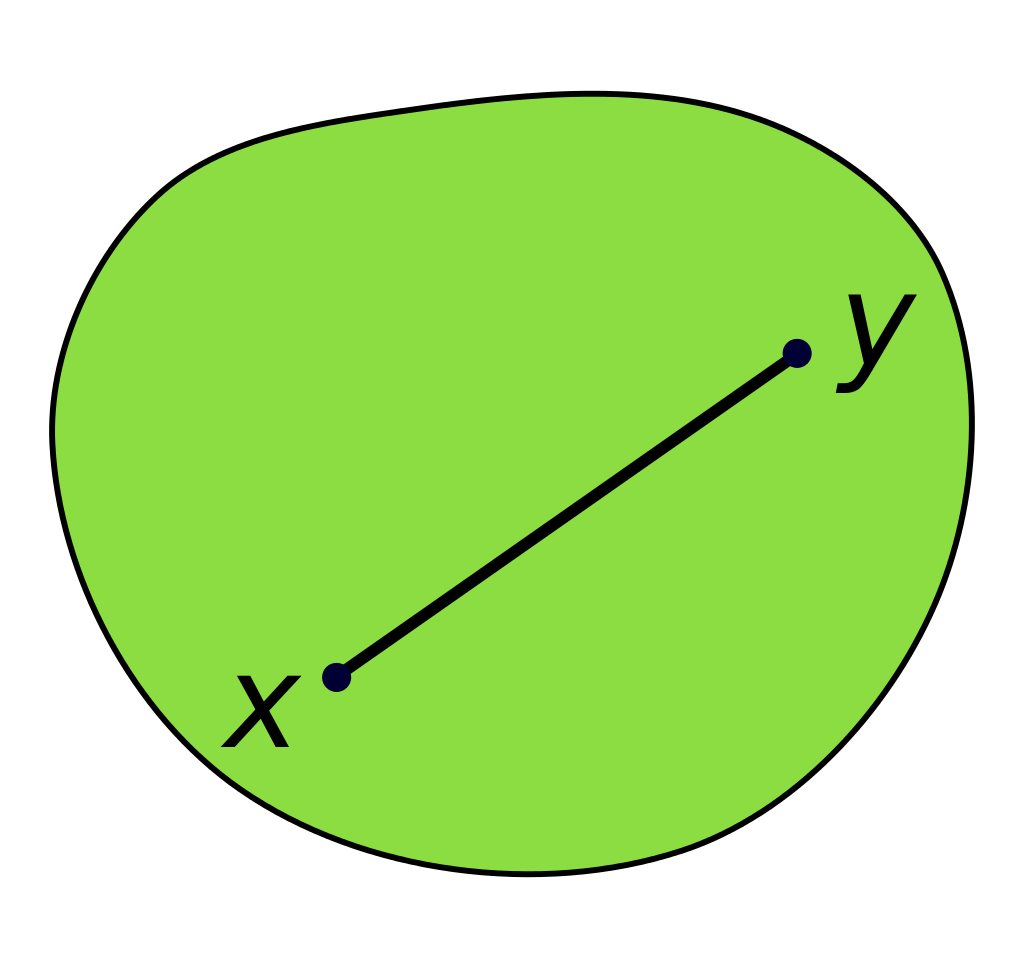
\includegraphics[width=0.8\textwidth]{figures/Convex_polygon_illustration1.png}
        \caption{Κυρτό Σύνολο}
        \label{fig:eg_convex_set}
    \end{subfigure}
    \hfill
    \begin{subfigure}[b]{.4\textwidth}
        \centering
        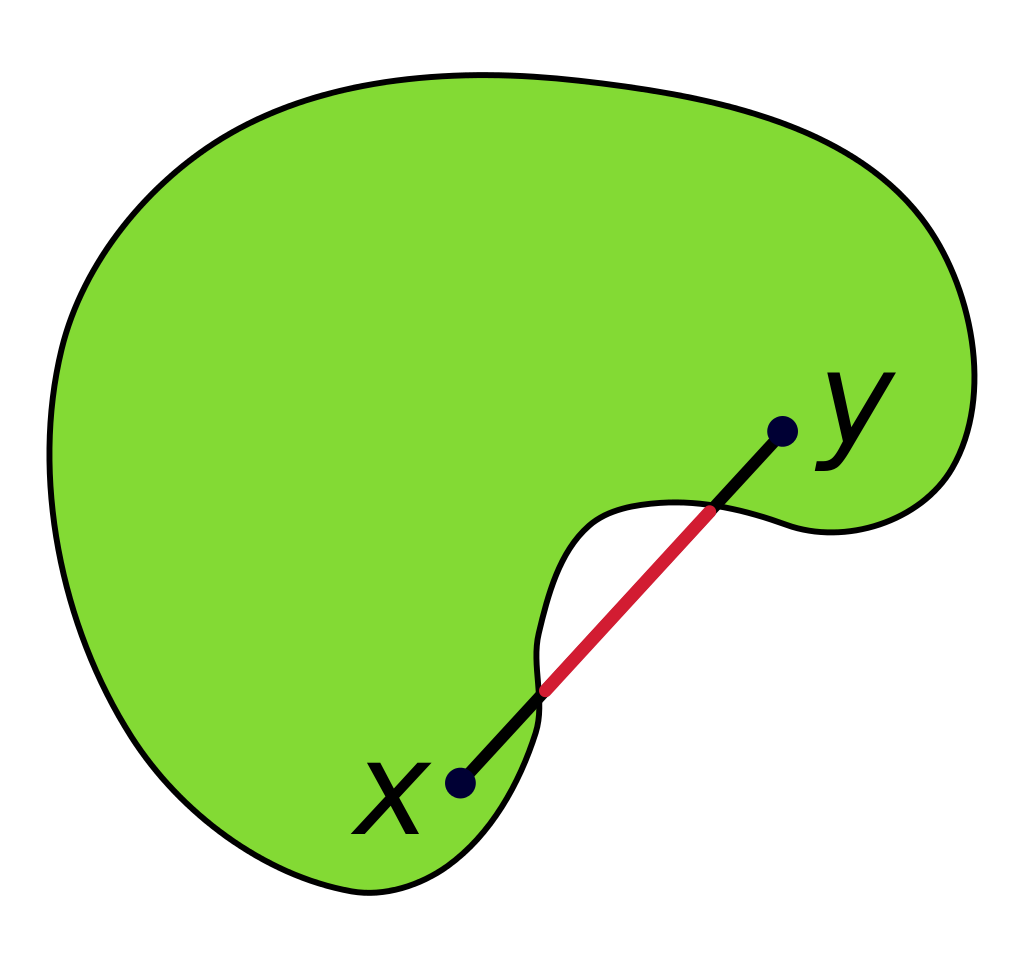
\includegraphics[width=0.8\textwidth]{figures/Convex_polygon_illustration2.png}
        \caption{Μη Κυρτό Σύνολο}
        \label{fig:eg_nonconvex_set}
    \end{subfigure}
    \caption{Κυρτά Σύνολα}
\end{figure}
\subsection{Κυρτό Σύνολο} Ένα σύνολο $C \subseteq \mathbf{R}^n$ ονομάζεται \textbf{κυρτό} αν το τμήμα
γραμμής μεταξύ δύο οποιοδήποτε σημείων που ανήκουν στο $C$, βρίσκεται στο
$C$. Για παράδειγμα αν για οποιοδήποτε $x_1, x_2 \in C$ και
$0 \leq \theta \leq 1$ τότε
\begin{equation*}
    x = \theta x_1 + (1 - \theta) x_2 \in C.
\end{equation*}

Ένα παράδειγμα κυρτού συνόλου παρουσιάζεται στο \ref{fig:eg_convex_set}, ενώ
αντιθέτως το σύνολο της \ref{fig:eg_nonconvex_set} δεν είναι κυρτό καθώς
μέρος του τμήματος της γραμμής μεταξύ των σημείων $x$ και $y$ δεν περιλαμβάνεται
στο σύνολο. Το σημείο της μορφής $\theta_1 x_1 + \dots + \theta_k
x_k$, όπου $\theta_1 + \dots + \theta_k = 1$ και $\theta_i \geq 0$ για $i = 1,
\dots ,k$, αναφέρεται ως \textbf{κυρτός
συνδυασμός} των σημείων $x_1 + \dots + x_k$. Το σύνολο όλων των κυρτών
συνδυασμών των σημείων του συνόλου $C \subseteq \mathbf{R}^n$
ονομάζεται \textbf{κυρτή θήκη} του $C$ και συμβολίζεται με
$\textbf{\tl{conv}} \ C$.

\subsection{Κυρτός κώνος} Το σύνολο $C$ ονομάζεται \textbf{κώνος}, αν για κάθε $x
\in C$ και $\theta \geq 0$ ισχύει ότι $\theta x \in C$. Το σύνολο $C$ είναι
\textbf{κυρτός κώνος} αν είναι κυρτό και κώνος, που σημαίνει ότι για οποιαδήποτε
$x_1, x_2 \in C$ και $\theta_1, \theta_2 \geq 0$ ισχύει
\begin{equation*}
    x = \theta_1 x_1 + \theta_2 x_2 \in C.
\end{equation*}
Στο σχήμα \ref{fig:convex_cone} παρουσιάζεται ένας κυρτός κώνος (ανοιχτό μπλε).
Μέσα σε αυτό, ο ροζ κυρτός κώνος αποτελείται από όλα τα σημεία
$\alpha x + \beta y$ με $\theta_1, \theta_2 \geq 0$.
\begin{figure}[h]
    \centering
    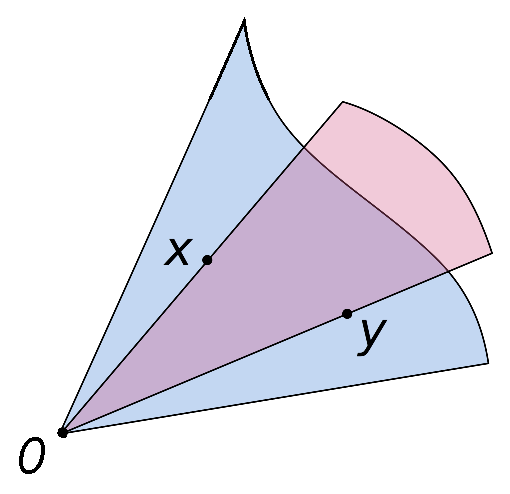
\includegraphics[scale=0.7]{figures/Convex_cone_illust.eps}
    \caption{Κυρτός Κώνος}
    \label{fig:convex_cone}
\end{figure}

\section{Σημαντικά Παραδείγματα}

\subsection{Υπερεπίπεδα} Ένα υπερεπίπεδο είναι ένα σύνολο της μορφής
\begin{equation*}
    \{ x \mid a^Tx = b \},
\end{equation*}
όπου $a \in \mathbf{R}^n, a \neq 0$ και $b \in \mathbf{R}^n$. Αναλυτικά είναι το
σύνολο λύσεων των γραμμικών εξισώσεων των συνιστωσών $x$. Γεωμετρικά το
υπερεπίπεδο μπορεί να ερμηνευτεί ως το σύνολο των σημείων με σταθερό εσωτερικό
γινόμενο ως προς το διάνυσμα $a$, ή ως το υπερεπίπεδο με κανονικό διάνυσμα
$a$, και η σταθερά $b$ καθορίζει την απόσταση του υπερεπιπέδου από την αρχή. Τα
υπερεπίπεδα είναι αφινικά και κυρτά.

\subsection{Ημιχώρος} Ένα υπερεπίπεδο χωρίζει το $\mathbf{R}^n$ σε δύο
\textbf{ημιχώρους}. Ένας (κλείστος) ημιχώρος είναι το σύνολο της μορφής
\begin{equation*}
    \{ x \mid a^Tx \leq b \},
\end{equation*}
όπου $a \neq 0$, π.χ., το σύνολο λύσης μίας ανισότητας. Οι ημιχώροι είναι κυρτοί
αλλά όχι αφινικοί.

\subsection{(Ευκλείδειες) Μπάλες} Μία \textbf{(Ευκλείδεια) μπάλα} στο $\mathbf{R}^n$
έχει τη μορφή
\begin{equation*}
    B(x_c, r) = \{x \mid \|x - x_c\|_2 \leq r\} = \{x \mid (x - x_c)^T(x - x_c) \leq
    r^2\},
\end{equation*}
όπου $r > 0$, και $\| \cdot \|_2$ συμβολίζει την Ευκλείδεια νόρμα. Το διάνυσμα
$x_c$ είναι το \emph{κέντρο} της μπάλας και το βαθμωτό μέγεθος $r$ η
\emph{ακτίνα} της.
Η μπάλα $B(x_c, r)$ αποτελείται από όλα τα σημεία που απέχουν το πολύ απόσταση
ίση με $r$ από το κέντρο $x_c$ και είναι κυρτό σύνολο.

\subsection{Ελλειψοειδές} Μία συγγενική κατηγορία κυρτού συνόλου είναι το
\textbf{ελλειψοειδές}, που περιγράφεται
\begin{equation*}
    \mathcal{E} = \{x \mid (x - x_c)^T P^{-1}(x - x_c) \leq 1\},
\end{equation*}
όπου $P = P^T > 0$, π.χ., το μητρώο $P$ είναι συμμετρικό και θετικά ορισμένο. Το
διάνυσμα $x_c \in \mathbf{R}^n$ είναι το \emph{κέντρο} του ελλειψοειδούς. Το
μητρώο $P$ καθορίζει κατά πόσο το ελλειψοειδές επεκτείνεται σε κάθε διεύθυνση
από το $x_c$. Το μήκος των ημιαξόνων του $\mathcal{E}$ δίνονται από τα
$\sqrt{\lambda_i}$, όπου $\lambda_i$ είναι οι ιδιοτιμές του $P$.

\subsection{Νόρμα} Μία συνάρτηση $\| \cdot \|$ που ικανοποιεί
\begin{itemize}
    \item $\|x\| \geq 0$ και $\|x\| = 0$ αν και μόνο αν $x = 0$,
    \item $\|tx\| = |t|\|x\|$ για κάθε $t \in \mathbf{R}$,
    \item $\|x + y\| \leq \|x\| + \|y\|$,
\end{itemize}
είναι \textbf{νόρμα}. Ο συμβολισμός $\| \cdot \|$ αποτελεί γενικό συμβολισμό,
συνήθως χρησιμοποιούμε κάποιο συμβολισμό για να προσδιορίσουμε τον τύπο της
νόρμας.

\subsection{Νορμική μπάλα και νορμικός κώνος} Θεωρώντας οποιαδήποτε νόρμα
$\| \cdot \|$ στο $\mathbf{R}^n$ και από τις ιδιότητες της νόρμας, η
\textbf{νορμική μπάλα} ακτίνας $r$ και κέντρου $x_c$ που περιγράφεται από
$\{ x \mid \|x - x_c\| \leq r\}$, είναι κυρτή. Ο \textbf{νορμκός κώνος}
εφοδιασμένος με τη νόρμα $\| \cdot \|$ είναι το σύνολο
\begin{equation*}
    C = \{(x,t) \mid \|x\| \leq t\} \subseteq \mathbf{R}^{n+1},
\end{equation*}
και είναι κυρτός κώνος.

\subsection{Πολύεδρα} Το \textbf{πολύεδρο} ορίζεται ως το σύνολο λύσης πεπερασμένων
γραμμικών ισοτήτων και ανισοτήτων:
\begin{equation*}
    \mathcal{P} = \{x \mid a_j^T x \leq b_j,\ j = 1, \dots, m,\ c_j^T x = d_j,\
    j = 1, \dots, p \}.
\end{equation*}
Το πολύεδρο είναι ουσιαστικά η τομή πεπερασμένων ημιχώρων και υπερεπιπέδων.
Αφινικά σύνολα (π.χ. υποχώροι, υπερεπίπεδα, γραμμές), τμήματα γραμμής και
ημιχώροι είναι όλα πολύεδρα. Επίσης, εύκολα αποδεικνύεται ότι τα πολύεδρα είναι
κυρτά σύνολα. Ένα φραγμένο πολύεδρο πολλές φορές καλείται \textbf{πολύτοπο}.
Πολλές φορές είναι βολική η συμπαγής μορφή του πολυέδρου
\begin{equation*}
    \mathcal{P} = \{x \mid Ax \leq = b, Cx = d\}.
\end{equation*}

\textbf{\tl{Simplexes}}. Τα \textbf{\tl{simplexes}} είναι μία
σημαντική κατηγορία πολυέδρων. Έστω τα $k + 1$ σημεία $v_0, \dots, v_k \in
\mathbf{R}^n$ είναι \textbf{αφινικά ανεξάρτητα}, που σημαίνει ότι $v_1 - v_0, \dots,
v_k - v_0$ είναι γραμμικώς ανεξάρτητα. Το \tl{simplex} τότε καθορίζεται από τη σχέση
\begin{equation*}
    \mathcal{C} = \textbf{\tl{conv}}\ \{v_0, \dots, v_k\} =
    \{ \theta_0 v_0 + \dots + \theta_k v_k \mid \theta \geq 0,\ \vc{1}^T\theta
    = 1\},
\end{equation*}
όπου το $\vc{1}$ συμβολίζει το διάνυσμα με όλα τα στοιχεία μονάδα. Η αφινική
διάσταση αυτού του συμπλέγματος είναι $k$, έτσι πολλές φορές λέγεται
$k$-διάστασης \tl{simplex} στο $\mathbf{R}^n$.

\textbf{Κυρτή θήκη και πολύεδρα}. Η κυρτή θήκη του πεπερασμένου συνόλου
$\{v_1,\dots,v_k\}$ είναι
\begin{equation*}
    \textbf{\tl{conv}}\ \{v_1,\dots,v_k\} = \{\theta_1 v_1+\dots+\theta_k v_k
    \mid \theta \geq 0,\ \vc{1}^T\theta = 1\}.
\end{equation*}
Το σύνολο αυτό είναι πολύεδρο και φραγμένο.

\subsection{Θετικά ημιορισμένος κώνος} Με το συμβολισμό $\mathbf{S}^n$ δηλώνουμε
το σύνολο των συμμετρικών $n \times n$ μητρώων,
\begin{equation*}
    \mt{S}^n = \{ X \in \mt{R}^{n \times n} \mid X = X^T\},
\end{equation*}
που είναι διανυσματικός χώρος διάστασης $n(n+1)/2$. Με το συμβολισμό
$\mathbf{S}_+^n$ δηλώνουμε το σύνολο των συμμετρικών θετικά ημιορισμένων μητρώων
\begin{equation*}
    \mt{S}_+^n = \{ X \in \mt{S}^{n} \mid X \geq 0\},
\end{equation*}
που είναι κυρτός κώνος και με το συμβολισμό $\mathbf{S}_{++}^n$ δηλώνουμε
το σύνολο των συμμετρικών θετικά ορισμένων μητρώων
\begin{equation*}
    \mt{S}_{++}^n = \{ X \in \mt{S}^{n} \mid X > 0\}.
\end{equation*}

\section{Πράξεις που διατηρούν την κυρτότητα}

\subsection{Τομή} Η κυρτότητα διατηρείται υπό την τομή συνόλων, αν $S_1$
και $S_2$ είναι κυρτά σύνολα, τότε η τομή $S_1 \cap S_2$ είναι κυρτή.
Η ιδιότητα αυτή επεκτείνεται για τομή απείρων συνόλων. Ένα απλό παράδειγμα
είναι το πολύεδρο που είναι η τομή ημιχώρων και υπερεπιπέδων, που είναι κυρτά,
και επομένως είναι κυρτό.

\subsection{Αφινικές συναρτήσεις} Μία συνάρτηση $f:\mathbf{R}^n \to \mathbf{R}^m$
είναι \textbf{αφινική} αν είναι το άθροισμα γραμμικών συναρτήσεων και σταθεράς.
Για παράδειγμα συνάρτηση της μορφής $f(x) = \mt{A}x + b$, όπου $\mt{A} \in
\mathbf{R}^{n\times m}$ και $b \in \mathbf{R}^m$. Έστω $S \subseteq
\mathbf{R}^n$ είναι κυρτό και $f:\mathbf{R}^n \to \mathbf{R}^m$ είναι αφινική
συνάρτηση. Τότε η εικόνα του $S$ υπό τον περιορισμό της $f$,
\begin{equation*}
    f(S) = \{ f(x) \mid x \in S\},
\end{equation*}
είναι κυρτή.Αντίστοιχα, αν $f:\mathbf{R}^k \to \mathbf{R}^n$ είναι αφινική
συνάρτηση, η αντίστροφη εικόνα του $S$ υπό τον περιορισμό της $f$,
\begin{equation*}
    f^{-1}(S) = \{ x \mid f(x) \in S\},
\end{equation*}
είναι κυρτή.Κάποια απλά παραδείγματα αφινικών συναρτήσεων είναι η
\textbf{κλιμάκωση} και η \textbf{μετατόπιση}. Αν $S \subseteq \mathbf{R}^n$
είναι κυρτό, $\alpha \in \mathbf{R}$ και $a \in \mathbf{R}^n$, τότε τα σύνολα
$\alpha S$ και $S + a$ είναι κυρτά, όπου
\begin{equation*}
    \alpha S = \{\alpha x \mid x\in S\}, \qquad S + a = \{x + a \mid x\in S\}.
\end{equation*}
Επίσης, το σύνολο λύσης \textbf{γραμμικών μητρώων ανισότητας}
(\tl{linear matrix inequality, LMI}), $\{x\mid A(x) \leq B\}$ είναι
κυρτό, όπου $B, A_i \in \mathbf{S}^m$.

\subsection{Γραμμική-κλασματική και προοπτική συνάρτηση}

\textbf{Συνάρτηση προοπτικής}. Ορίζουμε τη συνάρτηση προοπτικής $P :\
\mathbf{R}^n \to \mathbf{R}^n$, με πεδίο ορισμού $\textbf{\tl{dom}} \ P =
\mathbf{R}^n \times \mathbf{R}_{++}$, ως, όπου $\mathbf{R}_{++}$ δηλώνει το
σύνολο των πραγματικών θετικών αριθμών, $P(z, t) = z/t$. Η συνάρτηση αυτή
κλιμακώνει ή κανονικοποιεί διανύσματα ώστε η τελευταία συνιστώσα να γίνει μονάδα
και στη συνέχεια την αποβάλει. Το σημαντικό είναι ότι αν $C \subseteq
\textbf{\tl{dom}}\ P$ είναι κυρτό, τότε και η εικόνα
\begin{equation*}
    P(C) = \{P(x) \mid x \in C\},
\end{equation*}
υπό τη συνάρτηση προοπτικής είναι κυρτή. Επίσης, η αντίστροφη εικόνα ενός κυρτού
συνόλου υπό συνάρτηση προοπτικής είναι κυρτή, δηλαδή αν $C \subseteq
\mathbf{R}^n$ είναι κυρτό, τότε
\begin{equation*}
    P^{-1}(C) = \{(x, t) \in \mathbf{R}^{n + 1} \mid x/t \in C,\ t > 0\},
\end{equation*}
είναι κυρτή.

\textbf{Γραμμική-κλασματική συνάρτηση}. Μία \textbf{γραμμική-κλασματική
συνάρτηση} σχηματίζεται από τη σύνθεση συναρτήσεων προοπτικής με αφινικές
συναρτήσεις. Έστω $g: \ \mathbf{R}^n \to \mathbf{R}^{m+1}$ αφινική, π.χ.,
\begin{equation*}
    g(x) = \begin{pmatrix} A \\ c^T \end{pmatrix}x + \begin{pmatrix} b \\ d
    \end{pmatrix},
\end{equation*}
όπου $A \in \mathbf{R}^{m \times n}, b \in \mathbf{R}^m, c \in \mathbf{R}^n$,
και $d \in \mathbf{R}$. Η συνάρτηση $f: \ \mathbf{R}^n \to \mathbf{R}^{m}$,
δίνεται από $f = P \circ g$, η σύμφωνα με το παραπάνω παράδειγμα
\begin{equation*}
    f(x) = (Ax + b) / (c^Tx + d), \qquad \textbf{\tl{dom}}\ f = \{x \mid c^Tx + d >
    0\},
\end{equation*}
καλείται \textbf{γραμμική-κλασματική} (ή \textbf{προβολική}) συνάρτηση. Αν $c =
0$ και $d>0$, το πεδίο ορισμού της $f$ είναι το $\mathbf{R}^n$ και η $f$ είναι
αφινική συνάρτηση. Έτσι μπορούμε να θεωρήσουμε της αφινκές και τις γραμμικές
συναρτήσεις σαν ειδικές περιπτώσεις γραμμικών-κλασματικών συναρτήσεων. Όπως και
στην προηγούμενη περίπτωση, η εικόνα και η αντίστροφη εικόνα κυρτών συνόλων υπό
γραμμικών-κλασματικών συναρτήσεων είναι κυρτά σύνολα.

\section{Γενικευμένες ανισότητες}

\subsection{Γνήσιοι κώνοι και γενικευμένες ανισότητες} Ένας κώνος $K \subseteq
\mathbf{R}^n$ καλείται \textbf{γνήσιος κώνος} αν ικανοποιεί τα παρακάτω:
\begin{itemize}
    \item $K$ είναι κυρτό.
    \item $K$ είναι κλειστό.
    \item $K$ είναι στερεό, που σημαίνει ότι έχει μη-κενά εσωτερικά σημεία.
    \item $K$ είναι σημειακό (\tl{pointed}), που σημαίνει ότι δεν περιέχει καμία
        ευθεία (ή ισοδύναμα, $x \in K, -x \in K \Rightarrow x = 0$).
\end{itemize}
Ένας γνήσιος κώνος $K$ μπορεί να χρησιμοποιηθεί για να ορίσουμε τη
\textbf{γενικευμένη ανισότητα}, που είναι μερικώς διατεταγμένο στο
$\mathbf{R}^n$ και έχει πολλές ιδιότητες της τυπικής διατεταγμένης του
$\mathbf{R}$. Συνδέουμε με το γνήσιο κώνο $K$ το μερικώς διατεταγμένο σύνολο στο
$\mathbf{R}^n$ που ορίζεται από
\begin{equation*}
    x \leq {}_Ky \Leftrightarrow y - x \in K.
\end{equation*}
Επίσης, γράφουμε $x \geq_Ky$ για $y \leq_K x$. Αντίστοιχα, ορίζουμε την
\textbf{αυστηρή γενικευμένη ανισότητα} και συνδέουμε το γνήσιο κώνο με το
αυστηρό μερικώς διατεταγμένο σύνολο ως
\begin{equation*}
    x \leq_Ky \Leftrightarrow y - x \in \textbf{\tl{int}}\ K,
\end{equation*}
και γράφουμε $x >_K y$ για $y <_K x$. Κάποια τυπικά παραδείγματα είναι π.χ.
όταν $K = \mathbf{R}_+^n$, τότε η γενικευμένη ανισότητα $\leq_K$ αντιστοιχεί
σε ανισότητα ως προς την κάθε συνιστώσα μεταξύ διανυσμάτων: $x \leq_K y$
σημαίνει ότι $x_i \leq y_i$, για $i = 1, \dots, n$. Ακόμη, ο θετικά
ημιορισμένος κώνος $\mathbf{S}^n_+$ είναι ένας γνήσιος κώνος στο $\mathbf{S}^n$.
Η αντίστοιχη γενικευμένη ανισότητα $\leq_K$ είναι η ανισότητα μητρώων
$X \leq_K Y$ που σημαίνει ότι $Y - X$ είναι θετικά ημιορισμένο. Επίσης, οι
γενικευμένες ανισότητες $\leq_K$ έχουν όμοιες ιδιότητες με τη γνωστή ανισότητα
$\leq$ του $\mathbf{R}$.

\subsection{Ελάχιστο και ελαχιστοτικό στοιχείο} Ενώ πολλές από τις ιδιότητες των
γενικευμένων ανισοτήτων βρίσκονται σε αναλογία με αυτές του $\mathbf{R}$, αυτό
δεν συμβαίνει για όλες. Η πιο εμφανής διαφορά είναι ότι η $\leq$ στο
$\mathbf{R}$ είναι γραμμικώς διατεταγμένη, δηλαδή κάθε δύο σημεία είναι
συγκρίσιμα. Η ιδιότητα αυτή δεν ισχύει για τις γενικευμένες ανισότητες και αυτό
ως συνέπεια οι έννοιες του ελάχιστου και μέγιστου να χρήζουν ορισμού. Λέμε ότι
$x \in S$ είναι το \textbf{ελάχιστο} στοιχείο του $S$, σε σχέση με τη γενικευμένη
ανισότητα $\leq_K$, αν για κάθε $y \in S$ ισχύει $x \leq_K y$. Ορίζουμε το
\textbf{μέγιστο} στοιχείο του $S$, σε σχέση με τη γενικευμένη ανισότητα με τον
αντίστοιχο προφανή τρόπο. Αν ένα σύνολο έχει ελάχιστο (μέγιστο) στοιχείο, τότε
είναι μοναδικό. Μία παρόμοια έννοια είναι το \textbf{ελαχιστοτικό στοιχείο}
(\textbf{\tl{minimal element}}). Λέμε ότι $x \in S$ είναι το ελαχιστοτικό
στοιχείο του $S$, σε σχέση με τη γενικευμένη ανισότητα $\leq_K$,
αν $y \in S$ ισχύει $y \leq_K x$ μόνο όταν $y = x$. Αντίστοιχα για το
\textbf{μεγιστοτικό στοιχείο} (\textbf{\tl{maximal element}}).

\section{Υπερεπίπεδο διαχωριστικό και στήριξης}

\subsection{Θεώρημα διαχωριστικού υπερεπιπέδου} Έστω $C$ και $D$ μη-κενά ξένα κυρτά
σύνολα, δηλαδή $C \cap D = \emptyset$. Τότε υπάρχει $a \neq 0$ και $b$ τέτοια
ώστε $a^Tx \leq b$ για όλα τα $x \in C$ και $a^tx \geq b$ για όλα τα $x \in D$.
Με άλλα λόγια, η αφινική συνάρτηση $a^T x - b$ είναι μη-θετική στο $C$ και
μη-αρνητική στο $D$. Το υπερεπίπεδο $\{x \mid a^T x = b\}$ ονομάζεται
\textbf{διαχωριστικό υπερεπίπεδο} για τα σύνολα $C$ και $D$, ή λέμε ότι
\textbf{διαχωρίζει} το σύνολο $C$ και $D$. Σχηματικά το θεώρημα παρουσιάζεται
στο γράφημα \ref{fig:seperating_theorem}.
\begin{figure}[h]
    \centering
    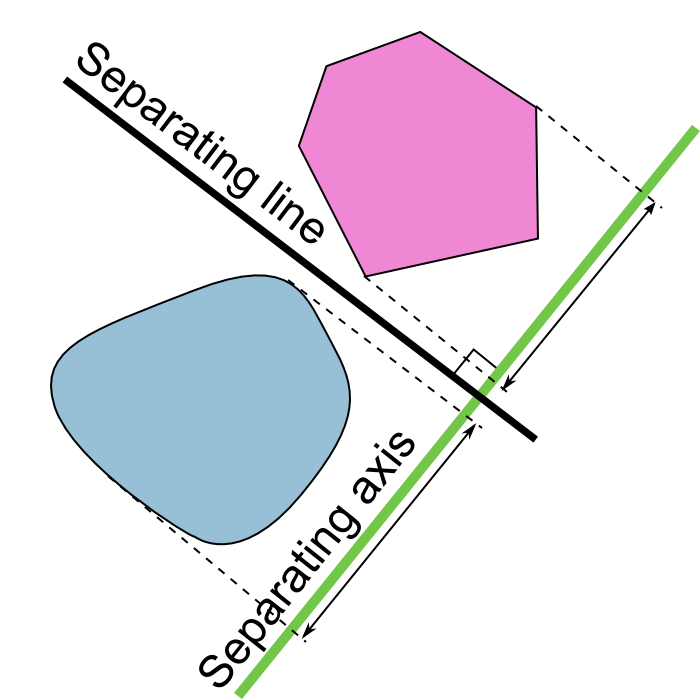
\includegraphics[scale=0.3]{figures/Separating_axis_theorem2008.png}
    \caption{Θεώρημα διαχωριστικού υπερεπιπέδου}
    \label{fig:seperating_theorem}
\end{figure}
Όπως ορίστηκε το παραπάνω θεώρημα, αν ισχύει μόνο η ανισότητα, και στις δύο
σχέσεις, τότε έχουμε το \textbf{αυστηρό διαχωριστικό υπερεπίπεδο}.

\subsection{Θεώρημα υπερεπιπέδου στήριξης} Έστω $C \subseteq \mathbf{R}^n$,
και $x_0$ είναι σημείο του συνόρου
\begin{equation*}
    x_0 \in \textbf{\tl{bd}}\ C.
\end{equation*}
Αν $a \neq 0$ ικανοποιεί $a^Tx \leq a^Tx_0$ για όλα τα $x \in C$, τότε το
υπερεπίπεδο $\{x \mid a^Tx = a^Tx_0\}$ ονομάζεται \textbf{υπερεπίπεδο στήριξης}
του $C$ στο $x_0$. Ισοδύναμα μπορούμε πούμε ότι το σημείο $x_0$ και το σύνολο
$C$ διαχωρίζονται από το υπερεπίπεδο $\{x\mid a^Tx = a^T x_0\}$. Γεωμετρικά,
όπως φαίνεται στο \ref{fig:supporting_theorem}, το υπερεπίπεδο είναι η εφαπτομένη του $C$ στο $x_0$ και ο
υποχώρος $\{x \mid a^Tx \leq a^Tx_0\}$ περιέχει το $C$.
\begin{figure}[h]
    \centering
    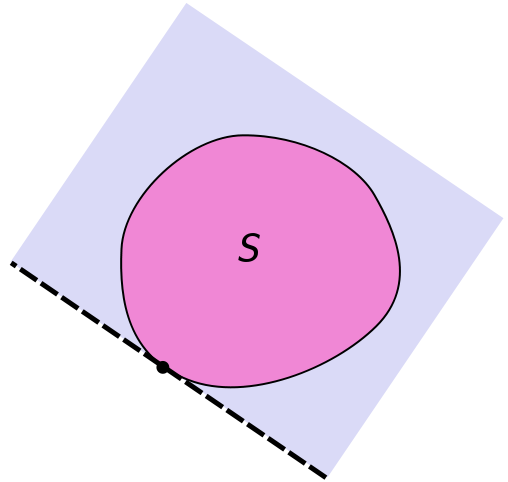
\includegraphics[scale=0.3]{figures/Supporting_hyperplane1.png}
    \caption{Θεώρημα υπερεπιπέδου στήριξης}
    \label{fig:supporting_theorem}
\end{figure}
Ένα βασικό αποτέλεσμα, που ονομάζεται \textbf{θεώρημα υπερεπιπέδου στήριξης},
δηλώνει ότι για κάθε μη-κενό κυρτό σύνολο $C$, και για οποιοδήποτε $x_0 \in
\textbf{\tl{bd}}\ C$, τότε υπάρχει υπερεπίπεδο στήριξης του $C$ στο $x_0$.

\section{Δυϊκός κώνος και γενικευμένες ανισότητες}

\subsection{Δυϊκός κώνος} Έστω $K$ κώνος. Το σύνολο
\begin{equation*}
    K^* = \{y \mid x^T y \geq 0 \ \text{για όλα τα} \ x \in K\}
\end{equation*}
ονομάζεται \textbf{δυϊκός κώνος} του $K$. Όπως υποδηλώνει το όνομα, $K^*$ είναι
κώνος και είναι πάντα κυρτός, ακόμα και αν ο κώνος $K$ δεν είναι. Για
παραδείγματα ο κώνος $\mathbf{R}^n_+$ είναι ο ίδιος δυΐκος
\begin{equation*}
    x^Ty \geq 0 \ \text{για όλα τα} \ x \geq 0 \Leftrightarrow y \geq 0
\end{equation*}
και λέμε τους κώνους αυτούς \textbf{αυτοδυϊκούς}.

\subsection{Δυϊκές γενικευμένες ανισότητες} Αν ο κυρτός κώνος $K$ είναι γνήσιος,
άρα επάγεται μία γενικευμένη ανισότητα $\leq_K$. Τότε ο δυϊκός κώνος είναι
επίσης γνήσιος, και επάγει μία γενικευμένη ανισότητα. Αναφερόμαστε στη
γενικευμένη ανισότητα $\leq_{K^*}$ ως τη \textbf{δυϊκή} της γενικευμένης
ανισότητας $\leq_{K}$. Μερικές σημαντικές ιδιότητες σχετικά με τη γενικευμένη
ανισότητα και την δυϊκή της είναι
\begin{itemize}
    \item $x \leq_K y$ αν και μόνο αν $\lambda^T x \leq \lambda^T y$ για κάθε
        $\lambda \geq_{K^*} 0$.
    \item $x <_K y$ αν και μόνο αν $\lambda^T x < \lambda^T y$ για κάθε
        $\lambda \geq_{K^*} 0$, $\lambda \neq 0$.
\end{itemize}

\subsection{Ελάχιστα και ελαχιστοτικά στοιχεία μέσω δυϊκών ανισοτήτων}

Χρησιμοποιώντας τις δυϊκές γενικευμένες ανισότητες μπορούμε να χαρακτηρίσουμε
ελάχιστα και ελαχιστοτικά στοιχεία (κυρτών ή όχι) συνόλων $S \subseteq
\mathbf{R}^m$ ως προς τις γενικευμένες ανισότητες που επάγονται από το γνήσιο
κώνο $K$.

\textbf{Δυϊκός χαρακτηρισμός ελάχιστου στοιχείου}. Το $x$ είναι
\textbf{ελάχιστο} στοιχείο του $S$, ως προς τη γενικευμένη ανισότητα $\leq_K$,
αν και μόνο αν για κάθε $\lambda >_{K^*} 0$, το $x$ είναι το μοναδικό που
ελαχιστοποιεί τη σχέση $\lambda^T z$ για $z \in S$. Γεωμετρικά, αυτό σημαίνει ότι για
κάθε $\lambda >_{K^*} 0$, το υπερεπίπεδο
\begin{equation*}
    \{z \mid \lambda^T(z - x) = 0\}
\end{equation*}
είναι ένα αυστηρό υπερεπίπεδο στήριξης του $S$ στο $x$. Αυστηρό
υπερεπίπεδο στήριξης σημαίνει ότι το υπερεπίπεδο τέμνει το $S$ μόνο
στο $x$. Η κυρτότητα του συνόλου $S$ δεν είναι απαραίτητη σύμφωνα με το
παραπάνω.

\textbf{Δυϊκός χαρακτηρισμός ελαχιστοτικού στοιχείου}. Αν το $x$ ελαχιστοποιεί
$\lambda^Tz$ για $z\in S$ και $\lambda >_{K^*} 0$ τότε το $x$ είναι
\textbf{ελαχιστοτικό}. Το αντίστροφο δεν ισχύει στη γενική περίπτωση, ένα σημείο
$x$ μπορεί να είναι ελαχιστοτικό του $S$, αλλά να μην ελαχιστοποιεί τη σχέση
$\lambda^Tz$ για $z\in S$ και οποιοδήποτε $\lambda$. Αν το σύνολο $S$
είναι κυρτό τότε για κάθε ελαχιστοτικό στοιχείο $x$ υπάρχει μη μηδενικό
$\lambda \leq_{K^*} 0$ τέτοιο ώστε το $x$ να ελαχιστοποιεί τη $\lambda^Tz$ για
$z\in S$.
